% !TEX TS-program = XeLaTeX
% use the following command:
% all document files must be coded in UTF-8
\documentclass[spanish]{textolivre}
% build HTML with: make4ht -e build.lua -c textolivre.cfg -x -u article "fn-in,svg,pic-align"

\journalname{Texto Livre}
\thevolume{19}
%\thenumber{1} % old template
\theyear{2026}
\receiveddate{\DTMdisplaydate{2026}{1}{29}{-1}} % YYYY MM DD
\accepteddate{\DTMdisplaydate{2026}{3}{22}{-1}}
\publisheddate{\DTMdisplaydate{2026}{10}{12}{-1}}
\corrauthor{Silvia Fernández Sabido}
\articledoi{10.1590/1983-3652.2026.64143}
%\articleid{NNNN} % if the article ID is not the last 5 numbers of its DOI, provide it using \articleid{} commmand 
% list of available sesscions in the journal: articles, dossier, reports, essays, reviews, interviews, editorial
\articlesessionname{articles}
\runningauthor{Fernández-Sabido y Peniche-Sabido} 
%\editorname{Leonardo Araújo} % old template
\sectioneditorname{Hugo Heredia Ponce~\orcid{0000-0003-3657-1369}}
\layouteditorname{Rayany Chaves~\orcid{0009-0007-0028-484X}}

\title{Soberanía tecnológica y lenguas indígenas: de la dominación histórica a la era de la inteligencia artificial}
\othertitle{Soberania tecnológica e línguas indígenas: da dominação histórica à era da inteligência artificial}
\othertitle{Technological sovereignty and indigenous languages: from historical domination to the era of artificial intelligence}
% if there is a third language title, add here:
%\othertitle{Artikelvorlage zur Einreichung beim Texto Livre Journal}

\author[1]{Silvia Fernández-Sabido~\orcid{0009-0009-8509-175X}\thanks{Email: \href{mailto:sfernandez@centrogeo.edu.mx}{sfernandez@centrogeo.edu.mx}}}
\author[2]{Laura Peniche-Sabido~\orcid{0009-0000-3680-3794}\thanks{Email: \href{mailto:penichesabidolaura@educativamexico.com.mx}{penichesabidolaura@educativamexico.com.mx}}}
\affil[1]{Secretaría de Ciencia, Humanidades, Tecnología e Innovación (Secihti), Centro de Investigación en Ciencias de Información Geoespacial (CentroGeo), Mérida, México.}
\affil[2]{Colegio “Educativa México”, Mérida, México.}

\addbibresource{article.bib}
% use biber instead of bibtex
% $ biber article

% used to create dummy text for the template file
\definecolor{dark-gray}{gray}{0.35} % color used to display dummy texts
\usepackage{lipsum}
\SetLipsumParListSurrounders{\colorlet{oldcolor}{.}\color{dark-gray}}{\color{oldcolor}}

% used here only to provide the XeLaTeX and BibTeX logos
\usepackage{hologo}

% if you use multirows in a table, include the multirow package
\usepackage{multirow}

% provides sidewaysfigure environment
\usepackage{rotating}

% CUSTOM EPIGRAPH - BEGIN 
%%% https://tex.stackexchange.com/questions/193178/specific-epigraph-style
\usepackage{epigraph}
\renewcommand\textflush{flushright}
\makeatletter
\newlength\epitextskip
\pretocmd{\@epitext}{\em}{}{}
\apptocmd{\@epitext}{\em}{}{}
\patchcmd{\epigraph}{\@epitext{#1}\\}{\@epitext{#1}\\[\epitextskip]}{}{}
\makeatother
\setlength\epigraphrule{0pt}
\setlength\epitextskip{0.5ex}
\setlength\epigraphwidth{.7\textwidth}
% CUSTOM EPIGRAPH - END

% to use IPA symbols in unicode add
%\usepackage{fontspec}
%\newfontfamily\ipafont{CMU Serif}
%\newcommand{\ipa}[1]{{\ipafont #1}}
% and in the text you may use the \ipa{...} command passing the symbols in unicode

% LANGUAGE - BEGIN
% ARABIC
% for languages that use special fonts, you must provide the typeface that will be used
% \setotherlanguage{arabic}
% \newfontfamily\arabicfont[Script=Arabic]{Amiri}
% \newfontfamily\arabicfontsf[Script=Arabic]{Amiri}
% \newfontfamily\arabicfonttt[Script=Arabic]{Amiri}
%
% in the article, to add arabic text use: \textlang{arabic}{ ... }
%
% RUSSIAN
% for russian text we also need to define fonts with support for Cyrillic script
% \usepackage{fontspec}
% \setotherlanguage{russian}
% \newfontfamily\cyrillicfont{Times New Roman}
% \newfontfamily\cyrillicfontsf{Times New Roman}[Script=Cyrillic]
% \newfontfamily\cyrillicfonttt{Times New Roman}[Script=Cyrillic]
%
% in the text use \begin{russian} ... \end{russian}
% LANGUAGE - END

% EMOJIS - BEGIN
% to use emoticons in your manuscript
% https://stackoverflow.com/questions/190145/how-to-insert-emoticons-in-latex/57076064
% using font Symbola, which has full support
% the font may be downloaded at:
% https://dn-works.com/ufas/
% add to preamble:
% \newfontfamily\Symbola{Symbola}
% in the text use:
% {\Symbola }
% EMOJIS - END

% LABEL REFERENCE TO DESCRIPTIVE LIST - BEGIN
% reference itens in a descriptive list using their labels instead of numbers
% insert the code below in the preambule:
%\makeatletter
%\let\orgdescriptionlabel\descriptionlabel
%\renewcommand*{\descriptionlabel}[1]{%
%  \let\orglabel\label
%  \let\label\@gobble
%  \phantomsection
%  \edef\@currentlabel{#1\unskip}%
%  \let\label\orglabel
%  \orgdescriptionlabel{#1}%
%}
%\makeatother
%
% in your document, use as illustraded here:
%\begin{description}
%  \item[first\label{itm1}] this is only an example;
%  % ...  add more items
%\end{description}
% LABEL REFERENCE TO DESCRIPTIVE LIST - END


% add line numbers for submission
%\usepackage{lineno}
%\linenumbers

\newenvironment{nobreakblock}{
    \par\vbox\bgroup
}{
    \egroup\par
}


\begin{document}
\maketitle

\begin{polyabstract}
\begin{abstract}
La relación entre las lenguas originarias y el desarrollo tecnológico ha estado históricamente marcada por tensiones de poder y exclusión sistémica. Este artículo analiza cómo la evolución de las tecnologías de la comunicación y la información reconfigura las relaciones de poder en las comunidades indígenas y condiciona su soberanía frente a la inteligencia artificial (IA). Mediante una revisión crítico-documental de 62 fuentes clave (67.7 \% de actualidad), apoyada en herramientas de IA para el soporte en la redacción, se sistematiza una genealogía que transita desde el saber ancestral hasta el activismo digital contemporáneo. Los resultados, sustentados en taxonomías de viabilidad técnica y evolución histórica que integran los impactos reportados en la literatura, revelan un movimiento pendular en la agencia tecnológica: desde la autonomía prehispánica hasta la desposesión simbólica mediante la alfabetización latina, culminando en la actual reapropiación de herramientas digitales y en el posicionamiento frente a los desafíos del Procesamiento de Lenguaje Natural (PLN). Se concluye que la integración soberana en los Grandes Modelos de Lenguaje (LLM) requiere trascender el extractivismo de datos para establecer protocolos de colaboración horizontal y diseño participativo. La soberanía de la palabra en la era de la IA es una condición necesaria para la alineación de la tecnología con los mejores valores humanos.

\keywords{Lenguas indígenas \sep Descolonización \sep Inteligencia artificial \sep Soberanía tecnológica \sep Tecnologías de la comunicación}
\end{abstract}

\begin{portuguese}
\begin{abstract}
A relação entre as línguas originárias e o desenvolvimento tecnológico tem sido historicamente marcada por tensões de poder e exclusão sistêmica. Este artigo analisa como a evolução das tecnologias da informação e comunicação reconfigura as relações de poder nas comunidades indígenas e condiciona sua soberania diante da inteligência artificial (IA). Por meio de uma revisão crítico-documental de 62 fontes fundamentais (67,7\% de atualidade), apoiada em ferramentas de IA para o suporte na redação, sistematiza-se uma genealogia que transita do saber ancestral ao ativismo digital contemporâneo. Os resultados, sustentados em taxonomias de viabilidade técnica e evolução histórica que integram os impactos relatados na literatura, revelam um movimento pendular na agência tecnológica: da autonomia pré-hispânica à despossessão simbólica mediante a alfabetização latina, culminando na atual reapropriação de ferramentas digitais e no posicionamento frente aos desafios do Processamento de Linguagem Natural (PLN). Conclui-se que a integração soberana nos Grandes Modelos de Linguagem (LLM) requer transcender o extrativismo de dados para estabelecer protocolos de colaboração horizontal e design participativo. A soberania da palavra na era da IA é, além de um direito indígena, uma condição necessária para o alinhamento da tecnologia com melhores os valores humanos.

\keywords{Línguas indígenas \sep Descolonização \sep Inteligência artificial \sep Soberania tecnológica \sep Tecnologias da comunicação}
\end{abstract}
\end{portuguese}


\begin{nobreakblock}
\begin{english}
\begin{abstract}
The relationship between Indigenous languages and technological development has been historically marked by power tensions and systemic exclusion. This article analyzes how the evolution of Information and Communication Technologies reconfigures power dynamics within Indigenous communities and how these dynamics condition their sovereignty in the face of Artificial Intelligence (AI). Through a critical documentary review of 62 key sources (67.7 \% of which were published between 2020-2026), supported by AI tools for writing assistance, a genealogy is systematized that moves from ancestral knowledge to contemporary digital activism. The results, supported by taxonomies of technical viability and historical evolution that integrate impacts reported in the literature, reveal a pendular movement in technological agency: from pre-Hispanic autonomy to symbolic dispossession through Latin literacy, culminating in the current re-appropriation of digital tools and positioning toward the challenges of Natural Language Processing (NLP). It is concluded that the sovereign integration of these languages into Large Language Models (LLMs) requires transcending data extractivism to establish protocols for horizontal collaboration and participatory design. Sovereignty over the spoken word in the era of AI is, in addition to an Indigenous right, a necessary condition for aligning technology with the best human values.

\keywords{Indigenous languages \sep Decolonization \sep Artificial intelligence \sep Technological sovereignty \sep Communication technology}
\end{abstract}
\end{english}
\end{nobreakblock}

% if there is another abstract, insert it here using the same scheme
\end{polyabstract}

\section{Introdución}\label{sec-intro}


\subsection{Panorama global de las lenguas indígenas}

En la actualidad, la identificación de quienes pertenecen a un pueblo indígena suele basarse en su lugar de residencia, lengua, vestimenta y costumbres, así como en su situación de marginación. Sin embargo, cuando una persona de origen indígena migra de un entorno rural a uno urbano se genera un proceso de adaptación en el que se mezclan elementos de la ruralidad con las nuevas experiencias de la ciudad, reconfigurando su identidad \cite{Corona2023}. En este escenario surgen preguntas interesantes: ¿Se deja de ser indígena al trasladarse a una ciudad y adoptar un estilo de vida diferente?, ¿Qué diríamos si la persona deja de usar su lengua y adopta la cultura del nuevo entorno?, ¿Qué sucede si, al intentar participar en la modernidad, simplemente no encuentra su lengua en internet? La poca presencia de las lenguas originarias en el mundo digital puede convertirse en una nueva forma de exclusión que obliga a elegir entre la herencia propia y la integración tecnológica.

Hoy día, menos del 6 \% de la población mundial se identifica como indígena \cite{Ivers2023}, lo que sugiere que cerca del 94 \% de la humanidad se ha alejado de su identidad originaria en diversos grados. La condición indígena parece ser un espectro que incluye desde personas que mantienen una conexión con su territorio, costumbres y lengua, hasta quienes han perdido su herencia cultural. De aquí surge otra pregunta: ¿Se puede recuperar la identidad perdida aprendiendo todos la lengua y cultura de nuestros ancestros?

Pese a que el Atlas Mundial de las Lenguas \cite{UNESCOWorldAtlasLanguages} reporta la pervivencia de cerca de 7 mil idiomas, su distribución y vitalidad son profundamente desiguales. Asia y África concentran la mayor diversidad lingüística, mientras que, en América Latina, países como México encabezan la lista con 68 lenguas originarias oficiales. Aunque la población indígena representa apenas el 6 \% mundial, este grupo resguarda el 60 \% de las lenguas del planeta y el 80 \% de su biodiversidad \cite{Ivers2023}. Este patrimonio se encuentra en estado de vulnerabilidad; solo el 0.8 \% de las lenguas documentadas son consideradas dominantes, mientras que la mayoría de las lenguas indígenas enfrentan riesgos de extinción.

\subsection{Sistemas de conocimiento originarios}

A pesar de que la vida de los pueblos originarios está permeada por tradiciones heredadas de la época colonial y moderna, aún se percibe un rico tapiz de saberes e idiomas ancestrales \cite{Mager2018,Makgopa2022} que revela su capacidad de sintetizar grandes campos de observación creando lo que ciertos autores denominan sistemas de conocimiento indígena \cite{Ajani2024,IbanezBlancas2020}. Estos sistemas abarcan los dominios de naturaleza y salud, extendiéndose hacia tecnología, sociedad, economía, cultura, gobernanza y educación.

Las lenguas indígenas codifican filosofías sobre la identidad territorial y la reciprocidad comunitaria, manteniendo el equilibrio entre el ser y su entorno. Estudios actuales demuestran que expresiones creativas modernas en lenguas originarias siguen cimentadas en filosofías ancestrales, como el \textit{Dalihan Na Tolu} en Indonesia \cite{Pasaribu2026}. Esta sabiduría se manifiesta en dimensiones prácticas; hoy día, estos pueblos conservan la habilidad de leer señales de anticipación climática, siguen interpretando signos del cuerpo ante una variedad de enfermedades y preservan formas de producción y alimentación orgánicas; resultado de miles de años de coevolución con su entorno, que presentan pocas externalidades negativas y requieren pocos insumos \cite{DeanceBravoTroncoso2017,Valladolid2007}.

Aunque no todos los individuos indígenas son conscientes de ese conocimiento, encontramos su impronta en las lenguas que usan. Por ejemplo, la lengua Maya tiene nombres para todas las partes del cuerpo, externas e internas, por pequeñas que sean. Ese saber es útil para el personal médico y de partería, sea indígena o no \cite{Janetsky2022,MartinBriceno2013}. Algunos pueblos utilizan formas de comunicación únicas, como silbidos o tañido de tambores que imitan el habla, con los que transmiten mensajes a larga distancia aprovechando las propiedades bioacústicas del entorno \cite{Meyer2012}. Ejemplos de ello son las comunidades silbos gomeros de las Islas Canarias, España, o la comunidad mazateca de Oaxaca, México, que se comunican con chiflidos compartiendo mensajes complejos que viajan kilómetros a través de la accidentada geografía de sus territorios.

La tecnología, entendida como el conjunto de técnicas reunidas en un sistema y tiempo determinados que se concretan en objetos físicos (Assess Technology, s/f), ha existido desde siempre. La tecnología ancestral indígena, como los sorprendentes pigmentos nanoestructurados \cite{FernandezSabido2012,Yacaman1996}, se caracteriza por estar adaptada al ambiente y ser útil en el contexto donde se gesta. Sin embargo, cuando la tecnología proviene del exterior, los beneficios para la comunidad suelen ser marginales.

\subsection{La brecha tecnológica y digital}

La desconexión entre el saber ancestral y la técnica externa adquiere una nueva dimensión en la era digital. Si lenguas como el maya poseen precisiones anatómicas que la ciencia convencional apenas comienza a integrar, su ausencia en los datos que alimentan la IA es una pérdida de conocimiento especializado que reduce la diversidad del pensamiento humano.

La tecnología no es neutral; afecta el bienestar colectivo y conlleva consecuencias políticas, ya que las relaciones de poder se entrelazan de manera inadvertida en su diseño y aplicación. El algoritmo es también un texto \cite{Araujo2025}, es decir, una construcción cargada de intencionalidad que, en el caso de las lenguas indígenas, suele imponer una visión monocultural. Estas dinámicas ocultas pueden generar injusticias sociales, lo que subraya la necesidad de reconocer cómo las herramientas tecnológicas inciden profundamente en la cultura resultando en una brecha profunda \cite{AlvarezAvila2016,Bielenberg1999}.

En México, los estados con mayor población indígena presentan los índices más bajos de conectividad y acceso a hardware \cite{INEGI2024}. Quienes no emplean lenguas dominantes quedan excluidos de los beneficios de la digitalización. Aunque han surgido estrategias de Educación Intercultural Bilingüe (EIB) y marcos legales robustos, como la Ley General de Derechos Lingüísticos en México o el reconocimiento del Estado Plural en Bolivia, persiste una desactualización normativa frente a las innovaciones tecnológicas.

La lengua constituye el vehículo primordial para acceder a los saberes ancestrales. La interacción \textit{lengua-sociedad} define todo un campo de estudio para las ciencias sociales, cuyo reto es dimensionar la pérdida epistémica que conlleva la extinción lingüística \cite{IbanezBlancas2020,RiosHernandez2010}. Ante esta amenaza, diversos actores han impulsado iniciativas para revertir el desplazamiento lingüístico, recurriendo a la tecnología para potenciar sus acciones.

\subsection{Evolución histórica de la agencia tecnológica indígena}

Mirar de cerca la relación entre los pueblos originarios y la tecnología, permite desmitificar la supuesta pasividad de estas comunidades frente a la innovación. Históricamente, la tecnología indígena no solo fue soberana, sino vanguardista; el desarrollo de materiales complejos como el Azul Maya \cite{FernandezSabido2012,Yacaman1996} y la sofisticación de sus sistemas de registro e inscripción \cite{Klein2001,Lenoir1998} demuestran una capacidad técnica autónoma donde lengua-herramienta operaban en una simbiosis epistémica. Sin embargo, la expansión colonial impuso marcos técnicos que reconfiguraron la tecnología como un instrumento de jerarquización y control \cite{Day2006,MallenRivera2012}, desplazando los saberes locales hacia la periferia del progreso. Pese a este desplazamiento, el siglo XXI ha sido testigo de una fase de reapropiación que se ha transformado en una estrategia de resistencia digital \cite{Dyson2016,Francese2023}.

Este trabajo presenta una revisión crítico-documental de los esfuerzos por integrar las lenguas y saberes de los pueblos originarios al ámbito tecnológico. El objetivo es, a partir de un análisis crítico de experiencias previas, mapear las tensiones, riesgos y oportunidades que surgen de la integración de las lenguas indígenas a la inteligencia artificial (IA). En particular, se examina su posición frente a los Grandes Modelos de Lenguaje (LLM, por sus siglas en inglés), donde la falta de representación amenaza con profundizar una brecha de invisibilidad digital. Es vital desplazar el enfoque desde la simple gestión de datos hacia procesos de intercambio humano; por ello, en este estudio se opta por el término “tecnologías de la comunicación y la información” sobre el concepto institucionalizado de “Tecnologías de la Información y la Comunicación” (TIC), reconociendo que la transmisión de saberes precede a lo técnico.

La presente investigación busca dar respuesta a la siguiente interrogante: ¿De qué manera la evolución de las tecnologías de la comunicación y la información ha reconfigurado las relaciones de poder en las comunidades indígenas, y cómo las tensiones entre la apropiación tecnológica y las estructuras de control histórico condicionan hoy su soberanía frente a la IA?

\section{Metodología}

La presente investigación adopta un enfoque cualitativo con un diseño documental y exploratorio, orientado a mapear la intersección entre las lenguas originarias y las tecnologías de la comunicación y la información. Se siguieron los principios generales de la declaración PRISMA para garantizar la transparencia y replicabilidad en la selección del corpus.

\subsection{Estrategia de búsqueda y consolidación del corpus}
El proceso de construcción del corpus se estructuró en dos etapas:

\begin{itemize}
    \item \textit{Recolección y curaduría}: se realizó una búsqueda en Dimensions-AI, ERIC, SciELO, Redalyc y Google Scholar. Se optó por estas fuentes debido a su alta pertinencia en lenguas originarias y contextos del Sur Global. Se utilizaron descriptores booleanos en español e inglés\textit{ tecnología AND lenguas indígenas}; \textit{indigenous languages AND technology}; \textit{procesamiento de lenguaje natural AND lenguas indígenas}).
    \item \textit{Validación de alto impacto y analítica de red}: se realizó una fase complementaria en Web of Science (WoS) y Scopus. Para robustecer la exhaustividad de la búsqueda y descubrir conexiones latentes entre autores del Sur Global, se empleó la herramienta de analítica de citas ResearchRabbit. Esta validación facilitó la integración de estudios de vanguardia (2024-2026) y aseguró una convergencia del 85 \% entre las fuentes detectadas.
\end{itemize}

\subsection{Criterios de selección y análisis situado}

De los 85 registros iniciales gestionados en Zotero, se aplicaron criterios de exclusión por redundancia teórica y pertinencia temática, resultando en un corpus de 62 documentos clave. La selección siguió un criterio temporal diferenciado: para el análisis de la IA y el Procesamiento de Lenguaje Natural (PLN), se aplicó un marco de vigencia (2020-2026) debido a la acelerada evolución de estas tecnologías. En contraste, para documentar la evolución histórica y la relación con las lenguas indígenas, se adoptó una perspectiva de largo alcance sin restricciones temporales. La distribución documental del corpus es: el 49.2 \% corresponde a artículos científicos, el 18.5 \% a libros y capítulos especializados, y el 13.8 \% a actas de congresos, complementados por informes de organismos internacionales (10.8 \%) y fuentes digitales (7.7 \%). El 67.7 \% de las fuentes pertenece al último lustro, manteniendo una representatividad predominante de México, América Latina y África, que refuerza un enfoque de investigación situado que refleja el origen de las autoras, quienes, como descendientes de pueblos originarios, asumen un compromiso personal con la visibilización de estas lenguas en el entorno digital.

\subsection{Uso de herramientas de asistencia}
En cumplimiento de las políticas de transparencia, se informa que se utilizaron los modelos de lenguaje Perplexity y Gemini como asistentes de redacción para la optimización de estilo y la traducción técnica de fragmentos específicos al inglés o portugués. La supervisión crítica, la verificación de fuentes y la autoría intelectual corresponden íntegramente a las investigadoras.

\section{Resultados}

La \Cref{tab1} sistematiza la evolución de las tecnologías de la comunicación y la información en contextos indígenas, vinculando cada fase con los impactos positivos y negativos reportados. Las herramientas se categorizan según su proveniencia (interna o externa), revelando que mientras las tecnologías externas históricamente han servido como vehículos de asimilación, las iniciativas internas tienden a fortalecer la cohesión comunitaria.

\begin{footnotesize}
\begingroup
\setlength{\tabcolsep}{3pt}
\begin{longtable}{
    >{\raggedright\arraybackslash}p{1.5cm}
    >{\raggedright\arraybackslash}p{2cm}
    >{\raggedright\arraybackslash}p{2cm}
    >{\raggedright\arraybackslash}p{2cm}
    >{\raggedright\arraybackslash}p{3cm}
    >{\raggedright\arraybackslash}p{3cm}
}
\caption{Evolución e impactos de las tecnologías de la comunicación y la información en contextos indígenas.}
\label{tab1}\\
% \toprule
% \textbf{Tecnología} &
% \textbf{Proveniencia (marca temporal)} &
% \multicolumn{2}{c}{\textbf{Agentes de creación y Ejemplos ejecución}} &
% \multicolumn{2}{c}{\textbf{Impacto reportado en comunidades indígenas}} \\
% &
% &
% &
% &
% \textbf{Positivo} &
% \textbf{Negativo} \\
\toprule
Tecnología &
Proveniencia (marca temporal) &
Agentes de creación y ejecución &
Ejemplos &
\multicolumn{2}{c}{Impacto reportado en comunidades indígenas} \\
& & & & Positivo & Negativo \\
\midrule
Escritura &
Interna (Pre-conquista) &
Especialistas indígenas en ciencia, tecnología y artes. &
Escritura en soportes variados: códices, cerámicas, piedra. &
Preservación de memorias históricas y sistemas de conocimiento
\cite{Chemla2005,FernandezSabido2012,Yacaman1996,Lenoir1998}. & \\

Escritura &
Externa (Siglo XVI) &
Iglesia y escuelas &
Libros impresos en papel con caracteres latinos. &
Acceso a la educación y al conocimiento
\cite{Bielenberg1999}. &
Evangelización y alfabetización masiva, deslegitimación de las culturas indígenas y exclusión de las mujeres de los registros oficiales de conocimiento
\cite{Bielenberg1999,Chemla2005,Day2006,GarcesVelasquez2020,Holmes2003,LlanesOrtiz2023,Janetsky2022}. \\

Navegación &
Interna (Pre-conquista) &
Personas artesanas, agricultoras y comerciantes indígenas. &
Navegación de rutas comerciales y ciclos astronómicos. &
Soberanía alimentaria y consolidación de redes de intercambio cultural
\cite{Valladolid2007,Yacaman1996}. & \\

Navegación &
Externa (Siglo XV) &
Potencias europeas &
Conquista transoceánica &
&
Pérdidas humanas, culturales y de territorio
\cite{Day2006,GutierrezFonseca2021,MallenRivera2012}. \\

Medios analógicos de comunicación &
Externa (Siglo XIX) &
Empresas productoras comerciales. &
Radio, cine y televisión &
&
Aumento de la brecha tecnológica, globalización que lleva a desaparecer tradiciones, reforzamiento de estereotipos
\cite{Cazden2003,Dyson2016,IturriagaAcevedo2020}. \\

Medios analógicos de comunicación &
Interna (Siglo XX) &
Agentes de comunicación indígena &
Radio, cine y televisión comunitarios &
Difusión de información en lenguas locales, producción educativa para proteger lenguas y culturas
\cite{Mkontwana2013,GobiernoMexico2023}. & \\

Tecnología digital &
Externa (Siglo XX) &
Grandes empresas tecnológicas y creadores de contenido del norte global . &
Internet, computadoras, dispositivos móviles, aplicaciones. &
&
Peligro para la diversidad lingüística, se difunden contenidos que favorecen culturas predominantes y debilitan identidades locales
\cite{AlvarezAvila2016,Cazden2003,GarcesVelasquez2020,LlanesOrtiz2023}. \\

Tecnología digital &
Interna (Siglo XXI) &
Activismo digital indígena: autorías musicales, artísticas y generadoras de contenido. &
Redes de telefonía, aplicaciones de celular, plataformas digitales, contenidos en redes sociales, doblaje de películas, diseño de tipografías. &
Preservación de sistemas de conocimiento indígena, revitalización de lenguas y culturas, descolonización del sistema educativo
\cite{Ajani2024,GarcesVelasquez2020,LlanesOrtiz2023,SolariPita2021}. & \\

Inteligencia artificial &
Externa (Siglo XXI) &
Grandes empresas tecnológicas e instituciones de investigación con incipiente participación indígena. &
Grandes modelos de lenguaje, asistentes virtuales, traductores. &
Surgen algunas aplicaciones de traducción y enseñanza de lenguas originarias, se abordan problemas étnicos y sociales de los pueblos indígenas
\cite{Caswell2024,Tonja2024}. &
Globalización acelerada, la brecha tecnológica se amplifica, personas indígenas relegadas a objetos de estudio y productoras de datos
\cite{Gasparotto2026,Joshi2020,Mager2018}. \\

Inteligencia artificial &
Interna (2020 - actualidad) &
Comunidades, personas lingüistas y tecnólogas indígenas. &
Proyectos de soberanía de datos, PLN comunitario. &
Empoderamiento, autogestión y diseño culturalmente situado
\cite{Araujo2025,HornaSaldana2025,Joshi2020}. &
Falta de recursos, dependencia de infraestructuras externas
\cite{Mager2018,Moraes2025}. \\
\bottomrule
\source{Elaboración propia a partir de las fuentes revisadas.}
\end{longtable}
\endgroup
\end{footnotesize}

 

Para comprender el contexto de vulnerabilidad en el que operan estas herramientas, en la \Cref{fig-1} se esquematizan las causas identificadas de la pérdida de las lenguas indígenas, destacando la presión de las lenguas hegemónicas y la brecha digital. Frente a este panorama, la \Cref{fig-2} ejemplifica diversas iniciativas que ilustran el alcance global del activismo digital indígena, mostrando una red de resistencia que ha ido trascendiendo las fronteras nacionales.

\begin{figure}[htbp]
\centering
\begin{minipage}{.8\textwidth}
 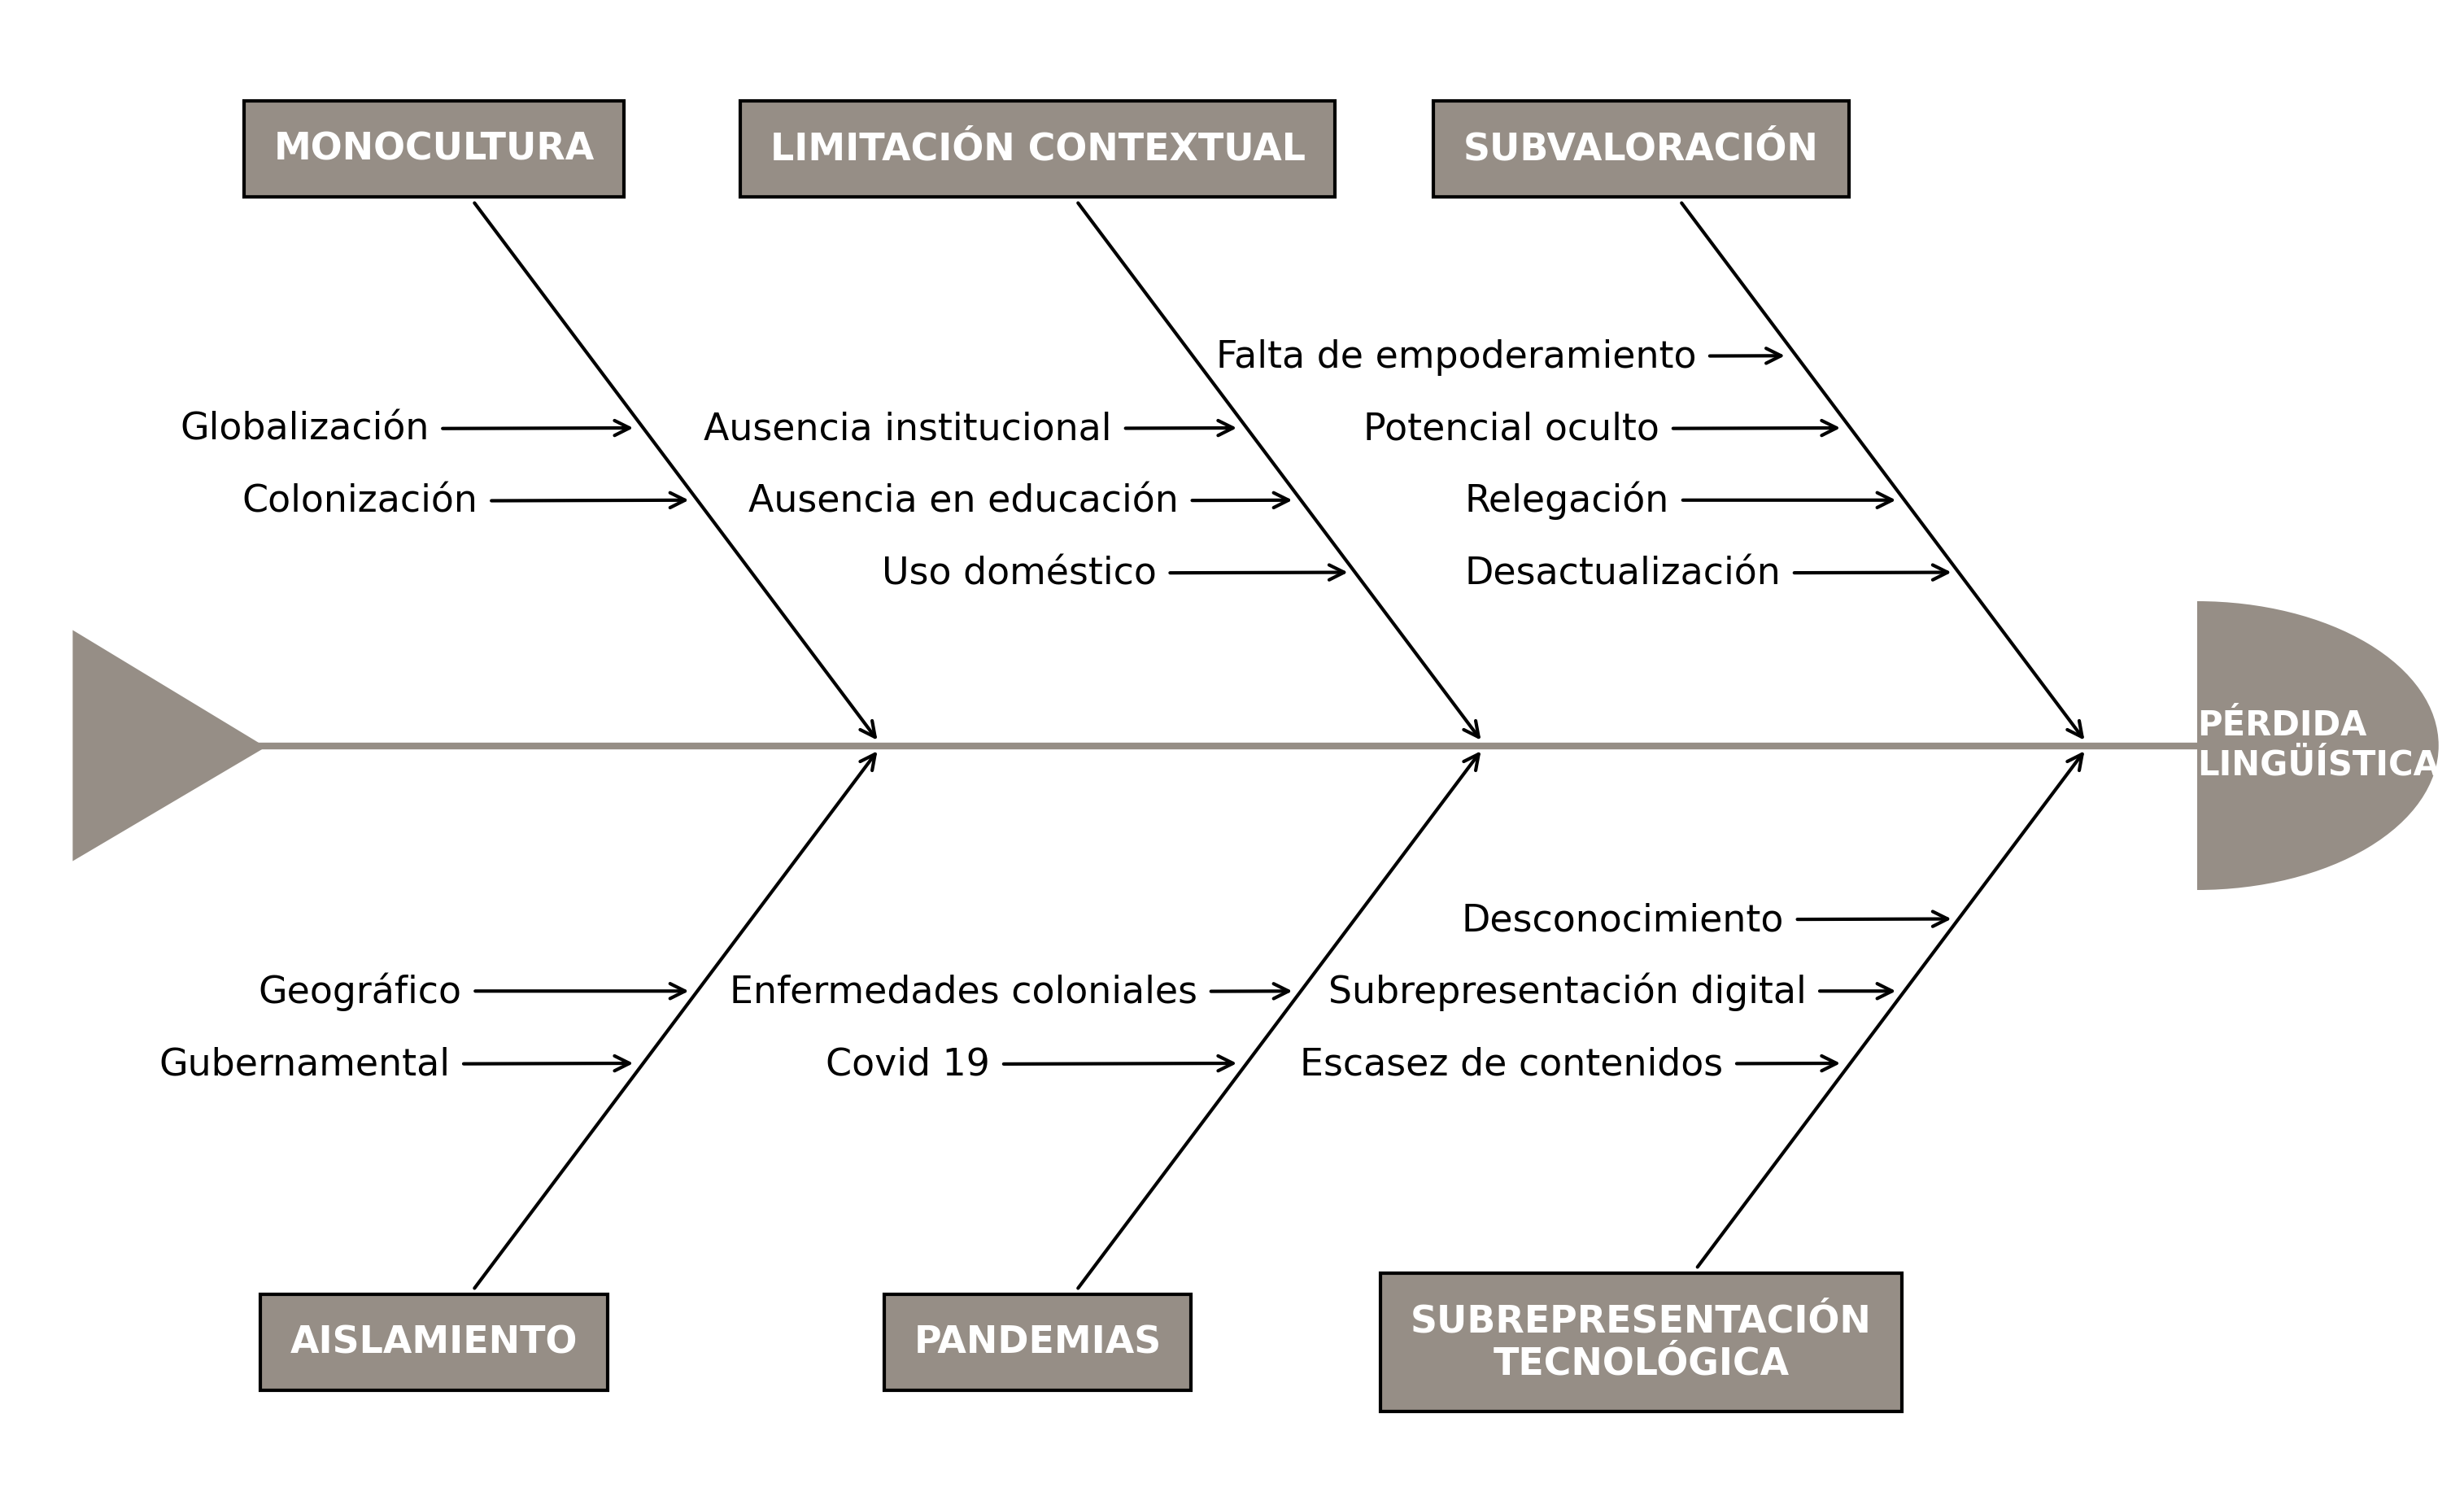
\includegraphics[width=\textwidth]{Fig1.png}
 \caption{Esquema de las causas identificadas de la pérdida de las lenguas indígenas.}
 \label{fig-1}
 \source{Elaboración propia a partir de los documentos citados en el texto.}
\end{minipage}
\end{figure}

La \Cref{tab2} presenta un contraste entre una lengua de recursos abundantes (holandés) y una de escasos recursos (somalí). Se evidencia la disparidad en la disponibilidad de datos para el entrenamiento de algoritmos, donde variables como la presencia en Wikipedia y la funcionalidad en sistemas de traducción marcan una brecha en la representatividad digital de los idiomas y una falta de estandarización deliberada.

La \Cref{tab3} propone una taxonomía actualizada de las herramientas de PLN para lenguas indígenas, clasificándolas según su viabilidad técnica. Se evidencia que la mayoría de estas lenguas se encuentran en una fase de recursos digitales fragmentarios, sin embargo, las nuevas estrategias de \textit{transfer learning} y modelos \textit{end-to-end} están permitiendo transitar hacia modelos de IA fomentando la autonomía comunitaria.


\begin{figure}[htbp]
\centering
\begin{minipage}{.8\textwidth}
 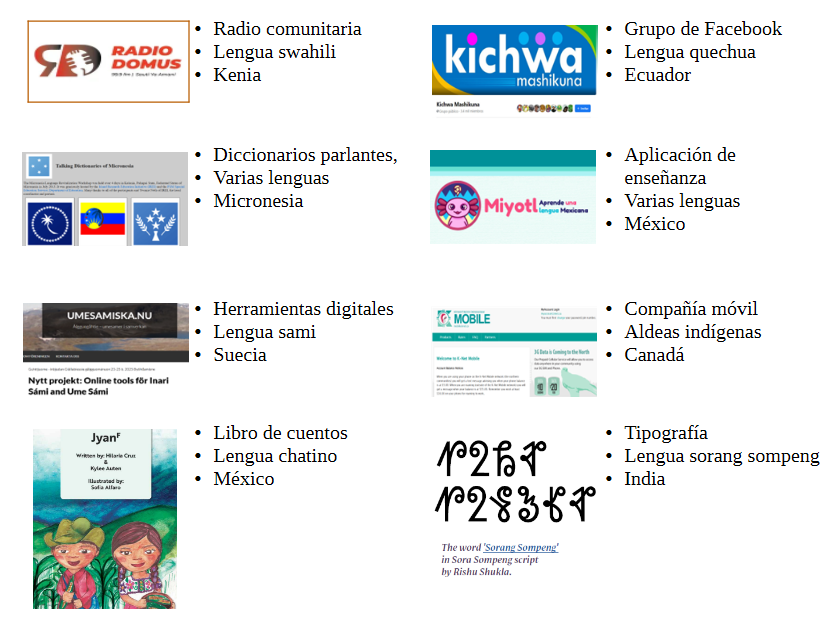
\includegraphics[width=\textwidth]{Fig2.png}
 \caption{Mosaico de iniciativas de activismo digital indígena.}
 \label{fig-2}
 \source{Elaboración propia a partir de fuentes revisadas. Imágenes tomadas de sitios oficiales (consultados en oct. 2024): Kenia (zeno.fm/radio/radio-domus-fm-kenya); Ecuador (facebook.com/groups/749828998458070); Micronesia (talkingdictionary.swarthmore.edu); México (proyecto-miyotl.web.app); Suecia (umesamiska.nu); Canada (mobile.knet.ca); México (ir.library.louisville.edu/chatino); India (commons.wikimedia.org/wiki/File:Shukla\_Sorang\_Sompeng.svg).}
\end{minipage}
\end{figure}



\begin{table}[htbp]
    \centering
    \renewcommand{\arraystretch}{1.3} 
    \small
    \caption{Disparidad entre una lengua con abundancia de recursos (high-resource) y otra de escasos recursos (low-resource).}
    \label{tab2}
    \begin{tabularx}{\textwidth}{
        >{\raggedright\arraybackslash}p{3cm} 
        >{\raggedright\arraybackslash}X 
        >{\raggedright\arraybackslash}X 
        >{\raggedright\arraybackslash}p{5cm}
    }
        \toprule
        Variable de comparación & 
        Holandés \newline (abundantes recursos) & 
        Somalí \newline (escasos recursos) & 
        Impacto de la falta de estandarización \newline \cite{Gasparotto2026} \\
        \midrule
        
        Población 
        & 29 millones 
        & 18 millones 
        & La demografía no dicta la prioridad tecnológica, sino la hegemonía del idioma. \\
        
        Presencia en Wikipedia 
        & 2 millones de artículos 
        & 5 mil artículos 
        & Los modelos se entrenan con sesgos de representatividad masiva. \\
        
        Uso en traducción 
        & Extensivo, alta calidad 
        & Calidad inferior 
        & Se imponen estructuras gramaticales externas que distorsionan el sentido. \\
        
        Ideología lingüística 
        & Estandarización global 
        & Invisibilización y fragmentación 
        & El PLN refuerza la exclusión al no reconocer variantes. \\
\bottomrule
\end{tabularx}
\source{Elaboración propia a partir del trabajo de \textcite{Mussandi2024}.}
\end{table}

%Ver por que a fonte está aparecendo como coluna

\begin{table}[htbp]
\centering
\caption{Clasificación y viabilidad de las tecnologías para lenguas indígenas.}
\label{tab3}
\small
\setlength{\extrarowheight}{3pt}
\begin{tabularx}{\textwidth}{>{\raggedright\arraybackslash}p{2.8cm} >{\raggedright\arraybackslash}X >{\raggedright\arraybackslash}X}
\toprule
Categoría & Disponibilidad real & Estado actual \\
\midrule

Emblemáticas \newline(traducción, Reconocimiento Automático de Voz [RAV]) & 
Baja funcionalidad, pero alta prioridad en investigación \cite{HornaSaldana2025}. & 
Basadas en \textit{transfer learning} y modelos \textit{end-to-end}. Se afinan con pocos datos, alta relevancia cultural. \\
\addlinespace

Prácticas \newline(teclados, búsqueda) & 
Amplia como metodología, pero limitada como tecnología. & 
Utilizan modelos pre-entrenados para normalizar la escritura reduciendo la influencia de estándares externos \cite{Gasparotto2026}. \\
\addlinespace

En espera \newline(ortografía, gramática) & 
Bloqueadas por falta de texto. Dependen del éxito de la transcripción automática. & 
La estrategia es usar el RAV para generar los volúmenes de texto necesarios para crear correctores. \\
\addlinespace

Experimentales \newline(IA Generativa, chatbots) & 
Prometedoras, pero su futuro está ligado al éxito de las categorías ``Emblemáticas'' y ``Prácticas''. & 
Avances, su éxito depende de la soberanía de los datos \cite{Moraes2025}. \\
\bottomrule
\end{tabularx}
\source{Elaboración propia adaptada de \textcite{Littell2018} con actualizaciones (2024-2026), a partir del trabajo de \textcite{Mussandi2024}.}
\end{table}


\section{Discusión}

\subsection{Genealogía tecnológica y lenguas indígenas}

La \Cref{tab1} revela un movimiento pendular en la agencia tecnológica indígena, marcando una transición desde la soberanía ancestral hacia la imposición colonial y el posterior retorno hacia la autonomía. Mientras que en el periodo pre-conquista la tecnología era de procedencia interna, la conquista (siglo XVI) desplazó la agencia hacia el exterior, convirtiendo la escritura y los medios analógicos en herramientas de deslegitimación. El punto de inflexión hacia la recuperación de la agencia se sitúa en el surgimiento del activismo digital. En este momento, las comunidades dejan de ser sujetos pasivos para convertirse en agentes que disputan el espacio virtual. Este retorno, iniciado con la reapropiación de las redes sociales y la creación de contenidos, se extiende hoy con la IA, que es el estadio más reciente de una soberanía tecnológica activamente en construcción. Para comprender la magnitud de esta recuperación, es preciso analizar cómo los soportes tecnológicos han condicionado la producción y el control de la información.

El papel ha sido una tecnología clave tanto en la producción de conocimiento \cite{Lenoir1998} como herramienta de dominación \cite{Day2006}. Pueblos originarios como mayas o egipcios lo usaron para registrar historias y conocimientos; sin embargo, el papel también es un dispositivo manipulable que sirve a intereses específicos \cite{Chemla2005,Holmes2003}. Esta ambivalencia sugiere que el soporte material del conocimiento nunca es neutro sino sujeto a las estructuras de poder de su época; como los algoritmos actuales, que al final son textos que proyectan intencionalidades en el espacio digital \cite{Araujo2025}.

La escritura moderna de las lenguas originarias de América, ajustada al sistema de la fuerza colonizadora (caracteres latinos), es una tecnología cuyo efecto no se considera del todo beneficioso \cite{GarcesVelasquez2020,LlanesOrtiz2023}. Un estudio con comunidades indígenas americanas, donde se implementaron campañas de alfabetización, concluyó que esta práctica altera la cultura que intenta preservar. Señala que el binomio iglesia-escuela ha sido el mayor promotor de la alfabetización indígena, con poco éxito fuera de estos ámbitos. Estas circunstancias han llevado a algunas comunidades a oponerse a la alfabetización, que prioriza la estructura del colonizador sobre los saberes propios \cite{Bielenberg1999}. Este proceso de alfabetización masiva fue una herramienta de desposesión simbólica. Al imponerse la escritura como único registro válido de la “verdad”, se invisibilizaron los saberes transmitidos por las mujeres indígenas, cuya autoridad reside tradicionalmente en la oralidad y la práctica comunitaria, tal como se observa en la discusión sobre partería de \textcite{Janetsky2022}.

La hegemonía del registro escrito no fue un fenómeno aislado. Las innovaciones tecnológicas han facilitado e intensificado las dinámicas de dominación sobre los pueblos indígenas y sus territorios: la invención de grandes embarcaciones permitió los viajes de conquista transoceánicos, mientras que las armas de fuego posibilitaron el sometimiento de civilizaciones enteras \cite{MallenRivera2012}.

La expansión tecnológica transitó desde la fuerza física hacia la influencia ideológica. Los primeros medios de comunicación masiva (radio, cine y televisión) contribuyeron a formar y deformar culturas. En Alaska se ha demostrado la relación entre la desaparición de tradiciones y la introducción de los televisores \cite{Cazden2003}. Aunque existen producciones televisivas encaminadas a proteger lenguas y culturas, también se han usado para estereotipar a las personas indígenas \cite{IturriagaAcevedo2020}, ejerciendo una suerte de extractivismo simbólico donde la imagen del indígena se utiliza sin su consentimiento o para fines ajenos a su bienestar.

La tecnología digital (internet, dispositivos móviles y computadoras) puede ser un peligro para la diversidad lingüística, ya que difunde contenidos que favorecen a las culturas dominantes y debilitan las identidades locales \cite{AlvarezAvila2016,GarcesVelasquez2020,LlanesOrtiz2023}. En este escenario, el riesgo se traslada al ámbito de los datos: el uso de lenguas indígenas en plataformas globales a menudo alimenta algoritmos externos sin que exista una retribución o protección para las personas hablantes. No obstante, la era digital también ha ofrecido una vía para la revitalización de los sistemas de conocimiento e idiomas indígenas \cite{Ajani2024}, siempre que la comunidad logre transitar desde el consumo pasivo hacia la soberanía tecnológica.

Finalmente, la IA representa la frontera más reciente de esta evolución tecnológica. Al igual que ocurrió con la escritura latina o la televisión, la IA no llega como una herramienta neutra. Los Grandes Modelos de Lenguaje (LLM) y los sistemas de traducción dependen de la recolección masiva de datos lingüísticos; sin embargo, cuando este proceso es liderado por entidades externas, se corre el riesgo de un extractivismo de datos, donde el conocimiento ancestral es procesado y monetizado sin el consentimiento o beneficio de las comunidades originarias \cite{Mager2018}. Pese a este peligro, como se sugiere en la \Cref{tab1}, la IA también abre la posibilidad de una tecnología de proveniencia interna. Si las comunidades lideran el desarrollo de sus propios modelos de Procesamiento de Lenguaje Natural (PLN), la IA puede dejar de ser una herramienta de asimilación para convertirse en un mecanismo de soberanía tecnológica que proteja y potencie la identidad indígena \cite{Joshi2020}.

\subsection{Causas estructurales de la erosión de las lenguas indígenas}
Como se muestra en la \Cref{fig-1}, la pérdida de las lenguas indígenas responde a una red de causas estructurales y desequilibrios de poder. El aislamiento geográfico y la falta de atención gubernamental limitan el acceso a servicios básicos, confinando las lenguas originarias al ámbito doméstico mientras las lenguas dominantes hegemonizan los espacios oficiales y académicos  \cite{Uekusa2019}. A este aislamiento se suman las catástrofes demográficas; desde la colonización hasta la pandemia de Covid-19, la pérdida de hablantes de edad avanzada ha fracturado la transmisión intergeneracional de conocimientos \cite{GutierrezFonseca2021}.


Asimismo, la subvaloración histórica ha desplazado los sistemas de conocimiento indígenas en favor de modelos europeos, un fenómeno que persiste en la actualidad \cite{GarcesVelasquez2020,Makgopa2022}. Aunque las revoluciones tecnológicas poseen un potencial democratizador, el vacío de contenidos digitales en lenguas originarias profundiza la brecha entre el desarrollo social y la adopción técnica \cite{DeanceBravoTroncoso2017,Joshi2020}. En la actual Cuarta Revolución Industrial (4IR), la IA amenaza con afianzar el dominio de pocos idiomas, a menos que se utilicen estos instrumentos para la emancipación mediante un enfoque multicultural y soberano \cite{Marwala2023}.


\subsection{Activismo digital indígena frente a la hegemonía técnológica}

Frente a las dinámicas de exclusión y dominación (\Cref{fig-1}), el activismo digital indígena surge como una gran fuerza de retorno hacia la soberanía. Este es un movimiento proactivo y, en gran medida, liderado por jóvenes, que busca descolonizar y democratizar la tecnología \cite{Marmion2014}. El fenómeno representa un ejercicio de soberanía tecnológica donde las comunidades retoman el control sobre sus propios datos, medios de comunicación y narrativas. La \Cref{fig-2} ejemplifica diversas iniciativas que ilustran este alcance a nivel global.

De manera notable, las radios comunitarias han desempeñado un papel fundamental en la difusión de información en lenguas locales, con un crecimiento constante en países como Sudáfrica \cite{Mkontwana2013} \cite{Omusonga2023} y México \cite{GobiernoMexico2023}. Asimismo, el uso estratégico de redes sociales ha permitido visibilizar movimientos de resistencia, como \#FeesMustFall en el sistema educativo sudafricano \cite{Tshifhumulo2021}. En contextos de revitalización, el pueblo Navajo en Estados Unidos utiliza estas plataformas para promover su cultura \cite{Reyhner2024}, mientras que en Ecuador se emplea Facebook para la difusión activa de la lengua quichua \cite{GarcesVelasquez2020}.

La creación de software y herramientas de aprendizaje autogestionadas es otro pilar del activismo. Los habitantes de la comunidad sami de Suecia personalizaron la aplicación Memrise para crear cursos de lengua \cite{LlanesOrtiz2023}, mientras que en México se han desarrollado múltiples aplicaciones para la enseñanza de lenguas nacionales \cite{MaldonadoRivera2018}. Estos esfuerzos se complementan con el desarrollo de infraestructura tipográfica, como la creación de fuentes para el sorang-sompeng en la India \cite{LlanesOrtiz2023} y proyectos similares en Latinoamérica \cite{SecretariaCultura2016}.

En el ámbito de la expresión artística y multimedia, el activismo se manifiesta en cómics tradicionales creados en Indonesia \cite{LlanesOrtiz2023}o en la música de jóvenes que utilizan internet para distribuir rap y hip-hop en lenguas originarias \cite{Francese2023}. Estos esfuerzos de reapropiación técnica alcanzan hitos como el desarrollo de recursos digitales para la lengua chatino por la lingüista Hilaria \textcite{Cruz2021}, o el primer doblaje de cine animado al matsigenka en Perú, promoviendo valores comunitarios y representación femenina \cite{SolariPita2021,LlanesOrtiz2023}.

Finalmente, el desarrollo de herramientas de productividad y conectividad refleja una búsqueda de autonomía técnica profunda. Los diccionarios parlantes de Micronesia \cite{LlanesOrtiz2023}, la suite ofimática TotoOffice en México, que permitió la redacción de una tesis académica en totonaco \cite{DeanceBravoTroncoso2017}, y el despliegue de redes de telefonía celular comunitaria en Canadá (Keewaytinook Mobile) y México (Tic-ac), demuestran que el activismo digital es capaz de ofrecer servicios esenciales a costos accesibles y bajo visiones propias \cite{Dyson2016,LlanesOrtiz2023}.

Los casos analizados son apenas una muestra de una agencia colectiva que prepara el terreno para el desafío tecnológico más sofisticado hasta la fecha: la IA. En esta transición, la lucha por la lengua se desplaza hacia la soberanía de los datos, convirtiéndose en el eje de las nuevas formas de activismo digital. Esta evolución se alinea con las tendencias actuales en la generación de textos dinámicos mediante LLM, los cuales, como sugieren \textcite{Ribeiro2025} en su reciente revisión sistemática, abren posibilidades inéditas para la producción de contenidos.

\subsection{Inteligencia artificial y la soberanía de datos indígenas}
El combustible principal de la IA son los datos (documentos, audios y videos) con los que se entrenan los modelos computacionales. Mientras las empresas tecnológicas los acumulan para crear aplicaciones que benefician a las lenguas dominantes, las lenguas indígenas quedan rezagadas \cite{Joshi2020,Tonja2024}. Esta desigualdad se hace evidente al contrastar dos idiomas con realidades digitales opuestas, tal como se ve en la \Cref{tab2} donde el PLN clasifica al somalí como “lengua de escasos recursos” y al holandés como “lengua de abundantes recursos” \cite{Mussandi2024}.

Es imperativo precisar que la etiqueta de “escasos recursos” es un término técnico-computacional que se refiere a la carencia de datos digitales y no a una precariedad del idioma. De hecho, las comunidades indígenas cuestionan este término por su connotación peyorativa, reivindicando que sus sistemas lingüísticos son ricos, efectivos y altamente complejos.

La falta de estandarización en el desarrollo del PLN refleja lo que \textcite{Gasparotto2026} identifica como ideologías lingüísticas dañinas. Al imponer normas de escritura y estructuras gramaticales ajenas, estos sistemas invisibilizan la riqueza de los idiomas originarios. De hecho, la fuerte oralidad de estos idiomas a menudo enmascara que muchas contaron con ingeniosos sistemas de escritura que se ajustan mejor a su fonología que la versión latina, cuya falta de simplicidad ha dificultado el aprendizaje y la producción de tecnología \cite{Joshi2020}.

Esta asimetría en la disponibilidad de recursos implica que las estrategias computacionales aplicadas a uno u otro grupo no son iguales pues las lenguas de escasos recursos presentan más desafíos. \textcite{Moraes2025} señalan que incluso en lenguas con abundantes datos, los modelos de lenguaje de gran escala enfrentan dificultades de ambigüedad lingüística que se agrava en idiomas con recursos digitales limitados donde la falta de contexto puede derivar en interpretaciones erróneas.

La diversidad lingüística y los fenómenos tipológicos de las lenguas indígenas presentan desafíos fascinantes para la ciencia \cite{GonzalezSantillan2021,Mager2018}. Salir de la cámara de resonancia tipológica, donde solo se exploran fenómenos de lenguas similares, permitirá enriquecer el campo del PLN \cite{Joshi2020,Ward2018}. Un estudio de \textcite{Littell2018} clasificó la viabilidad de estas herramientas en cuatro categorías; sin embargo, es preciso actualizar dicha taxonomía para reflejar los avances tecnológicos actuales (ver \Cref{tab3}).

Tradicionalmente, la falta de presencia digital ha limitado la viabilidad de las tecnologías para lenguas indígenas. No obstante, han nacido espacios académicos como NLPAméricas \cite{NLPA2021} y Africa Language Dataset Challenge \cite{AI4D2019} enfocados en crear materiales de investigación para lenguas como el guaraní, el bribri y el maya, así como generar datos de calidad en regiones de Ghana, Uganda y Sudáfrica \cite{Chiruzzo2024,Siminyu2021}.

El desplazamiento hacia tecnologías soberanas responde a la capacidad de optimizar algoritmos sin depender de volúmenes masivos de datos \cite{GonzalezSantillan2021,Joshi2020,Littell2018}. El paradigma técnico que lo permite es el aprendizaje por transferencia (transfer learning), que aprovecha el conocimiento de grandes arquitecturas multilingües para adaptar sistemas a lenguas indígenas mediante conjuntos de datos pequeños, pero de alta relevancia cultural.

La IA actúa como herramienta de archivo y como motor para cerrar la brecha de acceso a la información, permitiendo que los servicios digitales sean accesibles en lenguas nativas \cite{HornaSaldana2025}. Si bien empresas como Google han empleado estas técnicas para incluir lenguas como el n’ko de África, el punjabi de Pakistán, el manés de Irlanda y el maya yucateco de México \cite{Caswell2024}, su enfoque busca la cobertura global masiva más que la autonomía local.

Este camino resulta riesgoso pues al automatizar el proceso bajo lógicas externas, se corre el peligro de minimizar la participación de las personas hablantes, resultando en productos que carecen de interpretación cultural. El estado del arte apuesta por modelos end-to-end que logran la traducción de habla a habla permitiendo que la comunidad gestione su lengua como un fenómeno vivo y esencialmente oral. La verdadera innovación es la capacidad de las comunidades para gobernar estas herramientas \cite{Araujo2025}. El transfer learning solo es soberano si permite que los pueblos originarios dejen de ser proveedores de datos para convertirse en diseñadores de su futuro digital.

\section{Conclusiones}

En este trabajo se ha trazado un panorama sobre la compleja relación entre las lenguas indígenas y la evolución de las tecnologías de la comunicación y la información. El análisis evidencia que la pérdida de vitalidad lingüística es el resultado de tensiones de poder estructurales ligadas a la colonización y globalización, que han hecho necesaria la legislación de los derechos lingüísticos. El recorrido histórico permite concluir que la procedencia de la innovación técnica determina su impacto: cuando estas tecnologías son impuestas desde el exterior, suelen intensificar dinámicas de dominación; por el contrario, cuando son apropiadas y ejercidas desde la autonomía comunitaria, se transforman en instrumentos de resistencia con resonancia global.

La llegada de la IA plantea una encrucijada epistemológica. Si los modelos de lenguaje actuales son espejos de los valores depositados en internet, la exclusión de las lenguas originarias nos priva de sistemas de conocimiento y valores esenciales para el bienestar global. Esta exclusión no debe leerse como un fenómeno exclusivo de "lo indígena", ya que representa un síntoma de cómo el entrenamiento algorítmico tiende a marginar cualquier saber no hegemónico. Es imperativo que la incorporación de estas lenguas en la IA abandone el extractivismo de datos y se dirija hacia una investigación participativa que genere productos culturalmente pertinentes. Este proceso debe evitar la homologación de "lo indígena" como un bloque uniforme; como demuestra la hegemonía del quechua sobre lenguas como el puquina, la tecnología no debe replicar lógicas de expansión que erosionen la micro-diversidad de los territorios.

Cuando todas las lenguas humanas, con su carga de sabiduría milenaria, formen parte del tejido digital, tal vez surja, como una de las grandes capacidades emergentes de la tecnología, la tan buscada alineación de la IA con los mejores valores humanos. Esta alineación podría acompañarse de una toma de conciencia global donde cada individuo rastree su ancestría indígena para reencontrarse con la lengua y el territorio, constituyendo, tal vez, la campaña de revitalización más grande y efectiva.

Se reconoce que este estudio presenta limitaciones dadas por la celeridad del desarrollo de los LLM y la necesidad de profundizar en la literatura del Sur Global en otros idiomas, como el portugués; por ello, las taxonomías de viabilidad propuestas requieren actualización constante y validación empírica en territorios de baja conectividad. Hacia el futuro, es imperativo trascender el consentimiento informado convencional para establecer protocolos de colaboración horizontal. La verdadera soberanía digital solo será posible integrando a lingüistas y tecnólogos indígenas en los equipos de diseño, otorgando a la lengua un lugar central en la construcción del futuro tecnológico.





\printbibliography\label{sec-bib}
% if the text is not in Portuguese, it might be necessary to use the code below instead to print the correct ABNT abbreviations [s.n.], [s.l.]
%\begin{portuguese}
%\printbibliography[title={Bibliography}]
%\end{portuguese}


%full list: conceptualization,datacuration,formalanalysis,funding,investigation,methodology,projadm,resources,software,supervision,validation,visualization,writing,review
\begin{contributors}[sec-contributors]
\authorcontribution{Silvia Fernández-Sabido}[conceptualization,datacuration,formalanalysis,investigation,methodology,writing,review]
\authorcontribution{Laura Peniche-Sabido}[investigation,datacuration,writing,review]
\end{contributors}

\begin{dataavailability}
\txtdataavailability{databody} % options: dataavailable, dataonly, databody, datanotav, nodata
\end{dataavailability}

\begin{funding}
Este trabajo fue hecho en el marco de los proyectos INMX-4974 y CBF-2025-G-368 de la Secretaría de Ciencia, Humanidades, Tecnología e Innovación (SECIHTI) de México. 
\end{funding}




\end{document}

